\documentclass[11pt, a4paper]{article}

\usepackage[T1]{fontenc}
\usepackage[utf8]{inputenc}
\usepackage[UKenglish]{babel}
\usepackage{amsmath}
\usepackage{amsthm}
\usepackage{float}
\usepackage{graphicx}
\usepackage{algorithm}
\usepackage{algorithmic}
\usepackage{todonotes}
\usepackage{enumitem}

\newcommand{\nni}{\mathrm{NNI}}
\newcommand{\rnni}{\mathrm{RNNI}}
\newcommand{\rnniu}{\mathrm{RNNIu}}

\newtheorem{definition}{Definition}
\newtheorem{theorem}[definition]{Theorem}
\newtheorem{conjecture}[definition]{Conjecture}
\newtheorem{lemma}[definition]{Lemma}
\newtheorem{corollary}[definition]{Corollary}

\graphicspath{{figures/}}

\title{The Ranked Nearest Neighbour Interchange space}
\date{\today}
\author{Lena Collienne, Alex Gavryushkin}


\begin{document}

\maketitle

\begin{abstract}

\end{abstract}


\section{Introduction}

\section{Definitions}

%Do we restrict everything to RNNI? Make sure that we correctly distinguish between RNNI and RNNIu (for instance in the algorithm section)

%MRCA

%cluster

%leaf or taxon?

\begin{definition}
	Let $A$ be a pending subtree of the tree $T$.
	We call the set $c(A)$ of taxa of $A$ the \emph{cluster} induced by $A$.
\end{definition}

\section{Caterpillar Trees}

\begin{figure}[H]
	\centering
	\includegraphics[width=\textwidth]{NNI_vs_RNNI}
	\caption{Paths between caterpillar trees $T_1$ and $T_2$: black -- $\nni$ path of length $5$; red -- $\rnni$ path of length $6$; blue -- $\rnni$ path of length $8$.}
	\label{NNI_vs_RNNI}
\end{figure}

\begin{conjecture}
	The set of caterpillar trees is convex in $\rnni$ space.
\end{conjecture}

This conjecture is computationally proven for up to $8$ taxa (maximum $\rnni$ graph we can compute).
For a more restricted subset of trees in $\rnni$, namely caterpillar trees that have one cherry leaf in common, one can show convexity.

\begin{lemma}
	Let $T_1$ and $T_2$ be two caterpillar trees that both have a leaf labelled by $a$ as part of their cherry.
	There is a shortest paths from $T_1$ to $T_2$ that is a caterpillar path.
	\label{lemma:caterpillar_subset_convex}
\end{lemma}

\begin{figure}[h]
	\centering
	\includegraphics[width=0.3\textwidth]{label_internal_nodes}
	\caption{The labelling of the caterpillar tree as introduced in the proof of Lemma~\ref{lemma:caterpillar_subset_convex} is unique due to its definition.
	}
	\label{label_internal_nodes}
\end{figure}

\begin{proof}
	Let $T_1$ and $T_2$ be two caterpillar trees, both having a leaf labelled by $a$ as part of their cherry.
	Let $p$ be a shortest path from $T_1$ to $T_2$.
	We introduce a labelling of internal nodes of all trees on $p$ by first defining it for the caterpillar trees $T_1$ and $T_2$ and then explaining how the labelling is changed by $\rnni$ moves.

	In $T_1$ and $T_2$ the internal node of the cherry is labelled by the label of its child that is not $a$.
	All other internal nodes shall have the same label as their leaf children.
	From now on we will identify the leaf labelled by $x$ with $x$ and the internal node labelled by $x$ will be called $int_x$.
	An example for a caterpillar tree with internal leaf labels is depicted in Figure~\ref{label_internal_nodes}.
	In the following, changes of the internal labelling following $\rnni$ moves are defined:

	\textbf{Rank swaps:}
	Within rank swaps the labels of internal nodes do not change.
	For an example consider Figure~\ref{fig:rank_swap_internal_label}.

	\begin{figure}[H]
		\centering
		\includegraphics[width=0.8\textwidth]{rank_swap_internal_label}
		\caption{The labelling of the internal nodes that swap ranks (red) do not change within the rank swap.
		}
		\label{fig:rank_swap_internal_label}
	\end{figure}

	\textbf{NNI move:}
	Let there be an $\nni$ move on an edge $(int_x, int_y)$ where $rank(int_x) < rank(int_y)$ as in Figure~\ref{fig:nni_moves}.

	\begin{figure}[H]
		\centering
		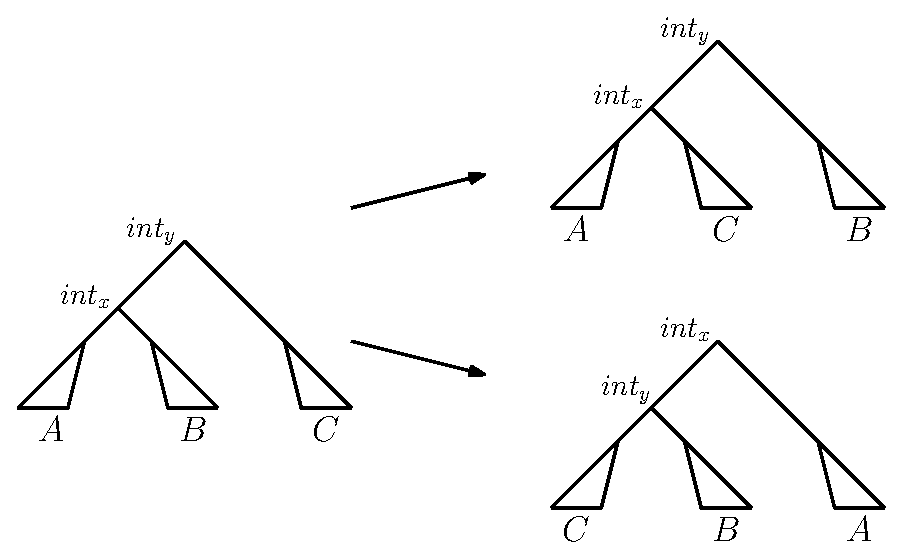
\includegraphics[width=0.7\textwidth]{nni_moves_internal_label}
		\caption{Two possible $\nni$ moves on edge $(int_x, int_y)$ where $x \in A, y \in B$.
		}
		\label{fig:nni_moves}
	\end{figure}

	The nodes incident to the edge after the $\nni$ move are labelled by $int_x$ and $int_y$ as well.
	By default, the node that has lower rank than the other one is labelled by $int_x$, the other one by $int_y$.
	But if $int_x$ is no ancestor of $x$ or $int_y$ is no ancestor of $y$, we swap the labels of the two new nodes, such that $rank(int_x) > rank(int_y)$.
	An example of an $\nni$ move and the new labelling is provided in Figure~\ref{fig:nni_example_internal_label}.

	\begin{figure}[H]
		\centering
		\includegraphics[width=0.8\textwidth]{nni_example_internal_label}
		\caption{The first labelling after the $\nni$ move preserves the ranks of $int_4$ and $int_6$.
		But then $int_6$ is not an ancestor of $6$ any more.
		Therefore, $int_4$ and $int_6$ have to change their labels.
		}
		\label{fig:nni_example_internal_label}
	\end{figure}

	We proceed to show that $int_x$ and $int_y$ are ancestors of $x$ and $y$ after an $\nni$ move as described above, respectively.
	If $x$ stays in the subtree rooted in the lower node of $e$, this does obviously hold.
	We now turn to the case that $x$ is not in the subtree rooted in the lower node of $e$ after the $\nni$ move.
	Then the labels of the two internal nodes change such that $rank(int_x) > rank(int_y)$.
	This makes sure that $int_x$ is an ancestor of $x$.
	Thus, it remains to prove that $int_y$ is ancestor of $y$.
	In particular, we need to show that $y$ is not in the same subtree $A$ as $x$, whose root has the node labelled by $int_x$ as parent before and after the $\nni$ move.
	Let us consider the tree before the $\nni$ move.
	$A$ has $|A|$ leaves and $|A| - 1$ internal nodes.
	These internal nodes are labelled by some leaves of $A$, because all internal nodes must be labelled by a descendant leaf.
	We know that $x \in A$, and the parent of the root of $A$ is labelled by $x$.
	All remaining $|A|-1$ leaf labels of $A$ appear as labels of the $|A|-1$ internal nodes of $A$.
	From the fact that the internal node labelled by $y$ is not inside $A$ we can conclude that $y$ cannot be a leaf of $A$.
	This proves that the labelling of the internal nodes is is well defined and allows a unique identification of internal nodes by their labels.

	The task is now to prove that there is always a caterpillar path at least as short as the given path $p$.
	Therefore, we use the following observation:
	Within each $\rnni$ move the ranks of at most two internal nodes change by at most one each.
	This is true for both rank swaps and $\nni$ moves, according to our definition of the labelling:
	Within a rank swap two nodes exchange their ranks, while there are not necessarily changes of ranks when $\nni$ moves are performed.

	On a caterpillar path the only possible moves are $\nni$ moves that change the ranks of two internal nodes by one each.
	Therefore, we can construct a caterpillar path $r$ out of $p$:
	every time two internal nodes $int_x$ and $int_y$ exchange ranks on $p$, they do so on the caterpillar path $r$ as well.
	Since there are moves on $p$ that do not change the ranks of internal nodes, this caterpillar path has length $|r| \leq |p|$.
	Hence, there is always a shortest path between $T_1$ and $T_2$ that is a caterpillar path.
\end{proof}

\section{Split Theorem}

When analysing the complexity of the $\rnni$ space, the comparison to $\nni$ is an important step.
The proof of NP-completeness of $\nni$ in~\cite{jiang2000} is based on the fact that following theorem holds in $\nni$.

\begin{theorem}
	There are trees $T_1,T_2$ in $\nni$ sharing a partition which is not shared by any intermediate tree on a shortest path from $T_1$ to $T_2$.
	\label{thm:split_nni}
\end{theorem}

\begin{proof}
	See~\cite{Li1996}.
\end{proof}

The proof presented in~\cite{Li1996} for Theorem~\ref{thm:split_nni} does not work for $\rnni$.

%This part is mainly for myself, not sure whether it is important to have it in the paper
The counterexample presented in~\cite{Li1996} works in $\nni$ is based on following observation:
Let $T_1$ and $T_2$ be two caterpillar trees.
If each taxon $a$ is replaced by a cherry $(a_1,a_2)$ in both trees $T_1$ and $T_2$, the resulting trees $T_1'$ and $T_2'$ have distance $d_{\nni}(T_1',T_2') = d_{\nni}(T_1,T_2)$ in the $\nni$ graph.
When proving~\ref{thm:split_nni},~\cite{Li1996} give an example of two trees $T$ and $R$ on $2n$ taxa that consist of two caterpillar trees each that share the root as parent.
The split given by the edges incident to the root is $1, \ldots, n | n+1, \ldots, 2n$ in both trees $T$ and $R$.
For the given example there is a shortest path in $\nni$ where at first $T$ is transformed to a tree $T'$ with $n$ cherries where each cherry contains one taxon of $\{1, \ldots, n\}$ and one taxon of $\{n+1, \ldots, 2n\}$.
Afterwards, $T'$ is tranformed to a tree $R'$ that contains the same cherries as $T'$.
Finally, all cherries of $R'$ are resolved in order to end up in tree $R$.
For proving that this path is shorter than any path preserving the split $1, \ldots, n | n+1, \ldots, 2n$, the fact that $d_{\nni}(T',R') = d_{\nni}(T|_{\{1, \ldots, n\}}, R|_{\{1, \ldots, n\}})$ is being used.
However, this does not work in $\rnni$.
Introducing new cherries means introducing new internal nodes with new ranks.
Since there are some rank swaps needed for an $\rnni$ path similar to the shortest $\nni$ path presented above, the path in $\rnni$ that breaks the split $1, \ldots, n | n+1, \ldots, 2n$ is no shortest path.
% How do we assign the ranks to the new cherry nodes?
% We could either create a path where $T'$ and $R'$ have distance equal to $d_{\rnni}(T|_{\{1, \ldots, n\}}, R|_{\{n+1, \ldots, 2n\}})$ and have a lot of additional rank swaps before and after that part OR
% Build $T'$ and $R'$ that contain all the cherries within the least number of moves possible (3n-3) and having a longer path between $T'$ and $R'$.
% Also anything in between these two options is possible. Are we able to disprove every option??


Therefore, the following conjecture was raised~\cite{Gavryushkin2017}.

\begin{conjecture}[Split Theorem]
	For the $\rnni$ graph the following statement holds:
	If a partition of leaves given by an edge is present in two trees $T$ and $R$ then the partition is presented in every tree on every shortest path between $T$ and $R$.
	\label{split_theorem}
\end{conjecture}

However, we found a counterexample to this conjecture:

\begin{figure}[H]
	\centering
	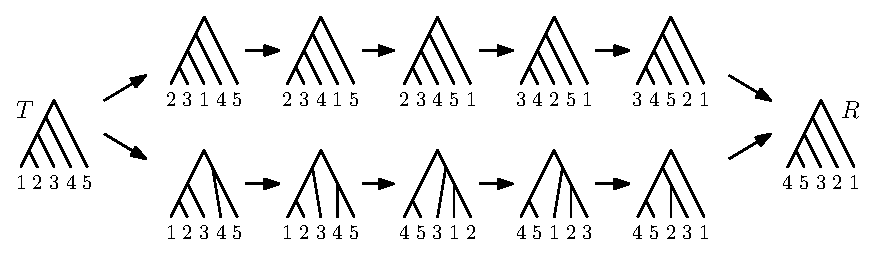
\includegraphics[width=\textwidth]{splitthm_counterexample}
	\caption{The split $123|45$ is present in $T_1$ and $T_2$, but the path at the top is a shortest path where none of the trees contains this split.
    However, this split is maintained on the path at the bottom that is a shortest path as well.}
	\label{splitthm_counterexample}
\end{figure}

Since the counterexample in Figure~\ref{splitthm_counterexample} clearly shows that the version of the Split Theorem stated in~\cite{Gavryushkin2017} does not hold, we will now claim an alternative to this conjecture.
The alternative formulation is based on the observation that there is a shortest path preserving all splits between the trees of the counterexample of the Split Theorem, which is presented at the bottom of Figure~\ref{splitthm_counterexample}.


\begin{conjecture}[Weak Split Theorem]
	For $\rnni$ graph the following statement holds:
	if a partition of leaves given by an edge is present in two trees $T$ and $R$ then there exists a shortest path between $T$ and $R$ where this partition is present in every tree on this path.
	\label{split_theorem_weak}
\end{conjecture}

\todo{Do we want to keep the weak version of the split thm? It is stronger than the Cluster Thm!}

% The weak Split Theorem (in the version as in Lena's thesis) is computationally proven to hold for trees with up to $6$ taxa ($\sim 38$ min running time on laptop).

Another alternative formulation of the Split Theorem is the \emph{Cluster Theorem}, which considers clusters instead of splits.
Considering clusters rather than splits is more reasonable since two rooted trees have the same set of clusters if, and only if, they are isomorphic~\cite{steel2016}.
The trees $T_1, T_2$ of counterexample~\ref{splitthm_counterexample} share the same set of induced splits, but have distinct sets of clusters.

\begin{conjecture}[Cluster Theorem]
	For the $\rnni$ graph the following statement holds:
	if two trees $T$ and $R$ contain the same cluster $C$, then $C$ is present as cluster in every tree on every shortest path between $T$ and $R$.
	\label{cluster_theorem}
\end{conjecture}


\section{Algorithms}

We are now going to introduce different algorithms that computes paths in $\rnni$.
\cite{Gavryushkin2017} gave an algorithm for computing the whole $\rnni$ space.
We implemented this algorithm and are able to use it on trees with up to $8$ taxa.
Therefore, we can compare the paths given by the algorithms presented in this chapter with the exact shortest path for trees with up to $8$ taxa.

% Shall we mention the data structure we use (list of sets) - this might be useful to see the connection to the partition lattice.

A modified version of the classic Bubble Sort \todo{cite} algorithm returns a caterpillar path that is shortest among all caterpillar paths between given caterpillar trees $T_1, T_2$.
Let $T_1 = (\ldots((1,2)3) \ldots )n), T_2 = (\ldots((\sigma_1,\sigma_2)\sigma_3) \ldots )\sigma_n)$ be two caterpillar trees.
They can be seen as sequences $(1,2,\ldots,n)$ and $(\sigma_1, \sigma_2, \ldots, \sigma_n)$ that need to be sorted.
$\nni$ moves between caterpillar trees correspond to exchanging two neighboured elements in a sequence.
The only exception of this are $\nni$ moves that change the cherry of a tree.
The corresponding moves on sequences are exchanged of either the second and third element or the first and third element.
On the other hand, there is no difference between two the trees corresponding to two sequences where only the first two taxa are exchanged.
Since all pairs of taxa whose order in $T_1$ is different from the one in $T_2$ need to be exchanged by $\nni$ moves on a caterpillar path, Bubble Sort will give a shortest path among all caterpillar paths.
Just the moves for the first three positions of the sequence must be adapted.
Let us consider the first three elements $(a,b,c,\ldots)$ of a sequence representing a caterpillar tree on a caterpillar path between $T_1$ and $T_2$
If the order of these elements is the same in $T_2$, there are no swaps needed for these taxa.
If just one of the two taxa $a$ and $b$ is on the other side of $c$ in $T_2$, this one will change wih $c$.
But if both $a$ and $b$ are on the other side of $c$ in $T_2$, the one which is the righmost of all three taxa in $T_2$ swaps with $c$ at first.
This makes sure that there is no additional swap of $a$ and $b$ needed on the path to $T_2$.
\todo{This paragraph is just a draft. Is it needed at all?}



Following algorithm computes paths between two trees in $\rnni$:

\begin{algorithm}[H]
\caption{FIND\_PATH($T_1,T_2$)}
\label{alg:find_path}
\begin{algorithmic}[1]
	\STATE $T := T_1$
	\STATE $p := (T_1)$
	\FOR {$r = 1, \dots, n-2$}
		\STATE Let $S$ be the cluster associated with the node $v$ in $T_2$ with $rank(v) = r$
		\WHILE {$rank(MRCA_T(S))>r$}
			\STATE Update $T$: Decrease $rank(MRCA_T(S))$ by an $\rnni$ move \label{alg:line:move_set_down}
			\STATE $p = p+T$
		\ENDWHILE
	\ENDFOR
	\RETURN p
\end{algorithmic}
\end{algorithm}

One can easily prove that there is always exactly one possible $\rnni$ move that decreases the rank of $MRCA_T(S)$ as in line~\ref{alg:line:move_set_down} of Algorithm~\ref{alg:find_path}.

The proof of Theorem 7 in \cite{Gavryushkin2017} gives an algorithm to compute paths between trees in $\rnni$.

% Compare the two algorithms by sampling trees and check which algorithm gives shorter paths.

% Also mention the exact algortihm for computing the whole RNNI space for up to 7 (?) taxa and check that Algorithm find_path gives correct distances there.
% Maybe it's worth trying the other algorithm in these trees as well.

Algorithm~\ref{alg:find_path} provides an upper bound for the diameter of $\rnniu$ space.
It improves the bound $n^2 - 3n - \frac{5}{8}$ given in \cite{Gavryushkin2017}.

\begin{theorem}
	It is $\Delta(\rnniu) \leq \frac{1}{2}n^2-\frac{3}{2}n+1$
\end{theorem}

\begin{proof}
	This result directly follows from Algorithm~\ref{alg:find_path}.
	In the worst case each $r = 1, \dots, n-2$ requires $n-1-r$ $\rnni$ moves for moving the corresponding $MRCA$ down.
	Hence, there is for each pair of trees a path of length less or equal to $\sum\limits_{i = 1}^{n-2} i = \frac{(n-2)(n-1)}{2} = \frac{1}{2}n^2-\frac{3}{2}n+1$.
\end{proof}

\begin{lemma}
	There are two caterpillar trees in $\rnniu$ with distance $\frac{1}{2}n^2-\frac{3}{2}n+1$.
	\label{conj:caterpillar_diameter}
\end{lemma}

\begin{proof}
    For this proof we will give two caterpillar trees $T_1$ and $T_2$ on $n$ taxa with $d_{RNNI}(T_1,T_2) = \frac{1}{2}n^2-\frac{3}{2}n+1$.
    \todo{$d$ or $d_{RNNI}$?}
	Let $T_1 = (( \dots (n,1)2)\dots)n-1)$ and $T_2 = (( \dots (n,n-1)n-2)\dots)1)$.
    According to Lemma~\ref{lemma:caterpillar_subset_convex}, there is a shortest path between $T_1$ and $T_2$ that only consists of caterpillar trees.
    We can compute such a shortest caterpillar path by using a modified version of Bubble Sort.
    When running this algorithm on $T_1$ and $T_2$ there are $n-1-i$ swaps of taxon $i$ with its right neighbour.
    Therefore, the total number of these swaps, and therefore $d_{RNNI}(T_1,T_2)$, is $\sum\limits_{i=1}^{n-1}(n-1-i) = \sum\limits_{i=0}^{n-2}i = \frac{1}{2}n^2-\frac{3}{2}n+1$
\end{proof}

\begin{corollary}
It is $\Delta(\rnniu) = \frac{1}{2}n^2-\frac{3}{2}n+1$.
\end{corollary}


\begin{lemma}
    Let $T$ be the caterpillar tree $(\ldots ((1,2),3), \ldots, n)$.\\
    A caterpillar tree $T'$ has distance $d(T,T') = \Delta(\rnniu) = \frac{1}{2}n^2-\frac{3}{2}n+1$ to $T$ if, and only if, $T' = ( \ldots ((n,t),n-1),n-2), \ldots, t+1), t-1) \ldots, 1)$
    \label{lemma:caterpillar_dist=diameter}
\end{lemma}

\todo{At the top of $T'$ it could also be $2,1$, or $t=1$}

\begin{figure}[H]
    \centering
    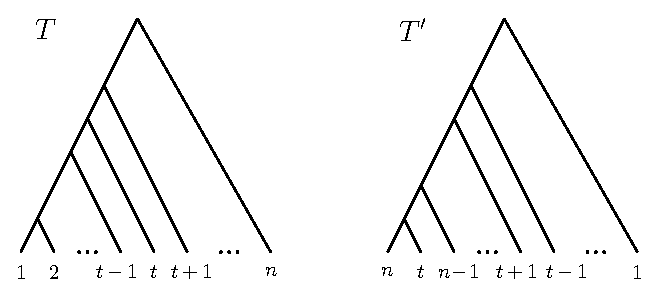
\includegraphics[width=0.6\textwidth]{caterpillar_max_dist}
    \caption{Caterpillar trees $T$ and $T'$ with distance $d(T,T') = \Delta(\rnniu)$}
    \label{fig:caterpillar_max_distance}
\end{figure}

\begin{proof}
    Let $T$ be the caterpillar tree $(\ldots ((1,2),3), \ldots, n)$.\\
    If $T'$ has distance $d(T,T') = \Delta(\rnniu)$ to $T$, is must be $T' = ( \ldots ((n,t),n-1),n-2), \ldots, t+1), t-1) \ldots, 1)$:

    Bubble Sort computes a shortest caterpillar path between two given trees.
    The maximum distance $\frac{(n-1)(n-2)}{2}$ can be reached by this algorithm, if in every loop every neighboured pair of taxa needs to swap.
    Starting at the tree $T$, this means that one of the taxa $1$ or $2$ moves up to the top of the tree in the first loop.
    In every consecutive loop one taxon in the cherry of the current tree that moves up in the tree and ends up directly below the taxon that was moved up in the previously loop.
    It is not hard to see that exchanging every neighboured pair of taxa as in Bubble Sort starting at $T$ leads to a tree $T'$ as described in the Lemma.
    The taxon $t$ is an arbitrary taxon of the set $\{1, \ldots, n-1\}$.
    If it is $1$, the uppermost taxon in $T'$ is $2$.
    These trees $T'$ are the only ones that need this maximum number of $\rnni$ moves starting at $T$.
    Therefore, it follows that $T' = ( \ldots ((n,t),n-1),n-2), \ldots, t+1), t-1) \ldots, 1)$ for every tree $T'$ with distance $d(T,T') = \Delta(\rnniu)$

    It remains to show that if $T' = ( \ldots ((n,t),n-1),n-2), \ldots, t+1), t-1) \ldots, 1)$, it follows that $d(T,T') = \Delta(\rnniu)$ to $T$.
    This can be proven by induction on the number of taxa $n$:

    Induction basis: $n=3$\\
    All trees have distance $1$.

    Induction step: $n \to n+1$\\
    Induction hypothesis: For trees $T_1 = (\ldots ((1,2),3), \ldots, n)$, $T_2 = ( \ldots ((n,t),n-1),n-2), \ldots, t+1), t-1) \ldots, 1)$ on $n$ taxa it is $d(T_1, T_2) = \frac{(n-1)(n-2)}{2} = \Delta(\rnniu_n)$.\\
    Let $T, T'$ be trees on $n+1$ taxa as described in the Lemma and a shortest path $p$ from $T$ to $T'$.
    Consider the trees $T|_n$ and $T'|_n$ that result from $T$ and $T'$ by deleting taxon $n+1$, respectively.
    Deleting taxon $n+1$ from all trees on $p$, and deleting all trees that appear more than once in a row, results in a path $p'$ from $T|_n$ to $T'|_n$.
    Applying the induction hypothesis onto $T|_n$ and $T'|_n$ shows that this path has length $\frac{(n-1)(n-2)}{2}$.
    We can now compare this new path $p'$ with $p$.
    The only steps that appear on $p$ but not on $p'$ are those involving the additional internal node.
    We can label this node by $n+1$ and define a bijection between the internal nodes in all trees on $p'$ and the corresponding nodes in the trees in $p'$.
    The additional internal node $n+1$ has rank $n$ in $T$ and ran $1$ in $T'$.
    Each $\rnni$ move can decrease the rank of a node by at most $1$.
    Therefore, there are at least $n-1$ $\rnni$ moves needed on $p$, which do not appear on $p'$, for moving the internal node $n+1$ down.
    Hence, it is $d(T,T') = |p| \geq n-1 + |p'| = n-1 + \frac{(n-1)(n-2)}{2} = \frac{n(n-1)}{2} = \Delta(\rnniu)$.
    Thus, there is a shortest path from $T$ to $T'$ that only consists of caterpillar trees.

\end{proof}

\begin{theorem}
    The set of caterpillar trees is convex.
\end{theorem}

\begin{proof}
    We prove the Theorem by induction on the length $l$ of a shortest caterpillar path between two caterpillar trees $T_1$ and $T_2$.

    Induction basis: $l = \Delta(\rnniu) = \frac{(n-1)(n-2)}{2}$\\
    With Lemma~\ref{lemma:caterpillar_dist=diameter} one can see that for each pair of caterpillar trees $T_1$, $T_2$ with distance $d(T_1,T_2) = \Delta(\rnniu)$ there is a caterpillar path from $T_1$ to $T_2$ between these trees.

    Induction step: $l+1 \to l$\\
    Induction hypothesis: For each pait of caterpillar trees with distance $l+1$ there is a shortest path between these trees that only consists of caterpillar trees.
    Let $T_1$ and $T_2$ be caterpillar trees with caterpillar distance $l$ \todo{define 'caterpillar distance'}.
    If $l \neq \Delta(\rnniu)$, there must be a pair of taxa $x,y$ that are neighboured in $T_2$ and have the same order in $T_1$ and $T_2$, which means that $rank(p_x) > rank(p_y)$ or $rank(p_x) < rank(p_y)$ holds in both trees $T_1$ and $T_2$.
    Then it follows that the tree $T_2'$ that equals $T_2$, but with exchanged taxa $x$ and $y$, has distance $l+1$ to $T_1$.
    So there must be a shortest path from $T_2'$ to $T_1$ that only consists of caterpillar trees.
    Since it does not matter in which order the pairs of taxa that need to exchange their position do exchange on a path between two caterpillar trees, $T_2$ is on a shortest caterpillar path from $T_2'$ to $T_1$.
    Therefore, it must be $d(T_1, T_2) = l$.

\end{proof}

\section{Partition lattice}

% Define Partition Lattice $\Pi_n$ and max chains in that lattice!

\begin{theorem}
	The $\rnni$ space on $n$ taxa is isomorphic to the space of maximum chains of the partition lattice $\Pi_n$ where two maximum chains are connected by an edge if, and only if, they differ by exactly one partition.
\end{theorem}

\bibliographystyle{abbrv}
\bibliography{lit}

\end{document}
